\usetikzlibrary{arrows.meta,chains,circuits.logic.US}

\tikzset{
    simple wire/.style={very thick,>=Latex},
    wire/.style={line width=1.5pt,>=Latex},
    wire small/.style={line width=1pt,>=Latex},
    binLabel/.style={font=\tt},
    hiBox/.style={red, very thick, draw},
    >=Latex,
}

\begin{frame}{circuits: gates}
    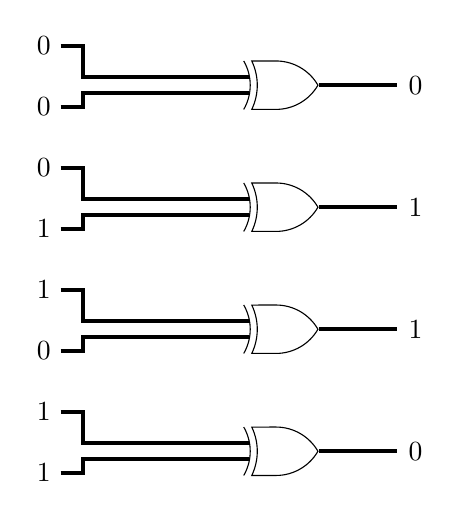
\begin{tikzpicture}[circuit logic US]
        \begin{scope}[start chain=inputs going below, every node/.style={on chain}, node distance=.3cm];
            \node {0};
            \node {0};

            \node {0};
            \node {1};

            \node {1};
            \node {0};

            \node {1};
            \node {1};
        \end{scope}
        \foreach \x/\y/\v in {1/2/0,3/4/1,5/6/1,7/8/0} {
            \node[xor gate] (xor-\x) at ([xshift=3cm,yshift=-.5cm]inputs-\x) {};
            \draw[wire] (inputs-\x) -- ++(.5cm,0cm) |- (xor-\x.input 1);
            \draw[wire] (inputs-\y) -- ++(.5cm,0cm) |- (xor-\x.input 2);
            \draw[wire] (xor-\x.output) -- ++(1cm,0cm) node[right] {\v};
        }
    \end{tikzpicture}
\end{frame}


